% Figure 1. The game as three nested loops, with the frames the model receives
% around them: the world map holds the locations, a location holds the battles
% that begin in it. Each frame points at the step it shows.
% Grid: 1 unit = 1 cm, four columns of W=3.25 with gap G=0.30 (13.90 wide).
% Rows: top frames (captions above), the band of loops, bottom frames
% (captions below). The band has the goal line and three nested boxes whose
% strips line up with columns 2, 3 and 4; column 1 of the band holds (g).
% Layers: z0 the boxes (fill darkens inward), z1 frames, z2 connectors, main
% all type.
\documentclass[tikz,border=1pt]{standalone}
\usepackage{times}
\usepackage[T1]{fontenc}
\usetikzlibrary{arrows.meta,calc}
\graphicspath{{.}{figures/}}

\definecolor{ink}{HTML}{1C1C1E}
\definecolor{accent}{HTML}{2F6FB0}
\definecolor{rule}{HTML}{DCDDE0}
\definecolor{wash}{HTML}{E8F0F8}
% depth as fill: world map, location, battle
\definecolor{d1}{HTML}{F4F5F7}
\definecolor{d2}{HTML}{E6E8EC}
\definecolor{d3}{HTML}{D6D9DF}
\definecolor{edge}{HTML}{8A8D93}

\newcommand{\W}{3.25}
\newcommand{\FH}{2.03}
\newcommand{\G}{0.30}
\newcommand{\C}{3.55}   % column pitch

\pgfdeclarelayer{z0}\pgfdeclarelayer{z1}\pgfdeclarelayer{z2}
\pgfsetlayers{z0,z1,z2,main}

\begin{document}
\begin{tikzpicture}[
  >={Stealth[length=1.8mm,width=1.3mm]},
  sub/.style={font=\rmfamily\footnotesize,text=ink,inner sep=0},
  title/.style={font=\sffamily\footnotesize\bfseries,text=ink,inner sep=0,anchor=north west},
  entry/.style={font=\sffamily\scriptsize,text=ink,inner sep=0,anchor=north west,align=left},
  link/.style={->,ink,line width=0.5pt,shorten >=1.2pt},
  loop/.style={->,ink,line width=0.6pt},
]
% ---------------------------------------------------------------- rows
\def\Ttop{-0.36}          % top of the top frames (caption above)
\def\Btop{-2.74}          % top of the band
\def\Bbot{-6.20}          % bottom of the band
\def\Ftop{-6.54}          % top of the bottom frames

% top frames: col 1 (c) axes, col 2 (b), col 3 (d), col 4 (a)
\foreach \col/\file/\nm/\cap in {%
  1/map-x3/fb/{(b) the world map},
  2/dialogue-x3/fd/{(c) dialogue, 16-pixel glyphs},
  3/room-x3/fa/{(d) the starting house}}
{
  \begin{pgfonlayer}{z1}
  \node[inner sep=0,anchor=north west] (\nm) at (\col*\C,\Ttop) {\includegraphics[width=\W cm]{\file}};
  \draw[rule,line width=0.4pt] (\nm.north west) rectangle (\nm.south east);
  \end{pgfonlayer}
  \node[sub,anchor=south west] at ($(\nm.north west)+(0,0.10)$) {\cap};
}
% bottom frames: col 1 (f), col 2 (h), col 3 (e), col 4 (i)
\foreach \col/\file/\nm/\cap in {%
  0/sheet-x3/ff/{(f) a character sheet},
  1/party-x3/fh/{(g) world-map menu and party},
  2/menu-x3/fe/{(h) the menu in a location},
  3/battle-x3/fi/{(i) a turn of a battle}}
{
  \begin{pgfonlayer}{z1}
  \node[inner sep=0,anchor=north west] (\nm) at (\col*\C,\Ftop) {\includegraphics[width=\W cm]{\file}};
  \draw[rule,line width=0.4pt] (\nm.north west) rectangle (\nm.south east);
  \end{pgfonlayer}
  \node[sub,anchor=north west] at ($(\nm.south west)+(0,-0.10)$) {\cap};
}
% band, column 1: (g) the inventory
\begin{pgfonlayer}{z1}
\node[inner sep=0,anchor=north west] (fg) at (0,\Btop-1.14) {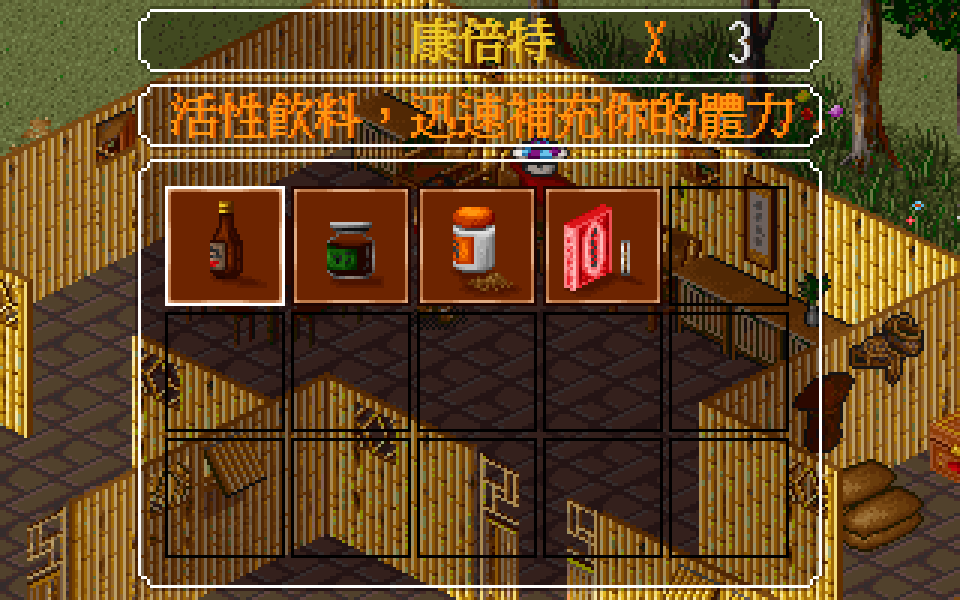
\includegraphics[width=\W cm]{inventory-x3}};
\draw[rule,line width=0.4pt] (fg.north west) rectangle (fg.south east);
\end{pgfonlayer}
\node[sub,anchor=north west] at ($(fg.south west)+(0,-0.10)$) {(e) the inventory};

% ---------------------------------------------------------------- (c) axes, top row col 1
\begin{scope}[shift={(0,\Ttop)}]
  \node[sub,anchor=south west] at (0,0.10) {(a) the four movement axes};
  \coordinate (o) at (\W/2, -\FH/2-0.05);
  \fill[wash] ($(o)+(0,0.40)$) -- ($(o)+(0.80,0)$) -- ($(o)+(0,-0.40)$) -- ($(o)+(-0.80,0)$) -- cycle;
  \draw[accent,line width=0.5pt] ($(o)+(0,0.40)$) -- ($(o)+(0.80,0)$) -- ($(o)+(0,-0.40)$) -- ($(o)+(-0.80,0)$) -- cycle;
  \fill[accent] (o) circle (0.06);
  \foreach \dx/\dy in {-1/1,1/1,-1/-1,1/-1}
    \draw[->,accent,line width=0.7pt] (o) -- ($(o)+(\dx*0.80,\dy*0.40)$);
  \foreach \dx/\dy/\k/\a in {-1/1/kp7/left,1/1/kp9/up,-1/-1/kp1/down,1/-1/kp3/right}{
    \node[font=\sffamily\scriptsize\bfseries,text=ink,inner sep=0,anchor=\ifnum\dx<0 east\else west\fi] at ($(o)+(\dx*0.86,\dy*0.52)$) {\k};
    \node[font=\sffamily\scriptsize,text=ink,inner sep=0,anchor=\ifnum\dx<0 east\else west\fi] at ($(o)+(\dx*0.86,\dy*0.52-0.26)$) {\a};
  }
  \coordinate (fc) at (\W-0.05,-\FH+0.12);
\end{scope}

% ---------------------------------------------------------------- the band
% the goal, band column 1, above (g)
\node[entry,anchor=north west,text width=\W cm,align=flush left] (goal) at (0,\Btop-0.10)
  {\footnotesize\textbf{Goal}\ \ the fourteen books, then the final battle and the ending};

\def\Wtop{\Btop}
% nested boxes
\begin{pgfonlayer}{z0}
  \draw[edge,fill=d1,rounded corners=3pt,line width=0.5pt] (\C,\Wtop) rectangle (4*\C-\G,\Bbot);
  \draw[edge,fill=d2,rounded corners=3pt,line width=0.5pt] (2*\C-0.12,\Wtop-0.10) rectangle (4*\C-\G-0.10,\Bbot+0.10);
  \draw[edge,fill=d3,rounded corners=3pt,line width=0.5pt] (3*\C-0.12,-4.04) rectangle (4*\C-\G-0.20,\Bbot+0.20);
\end{pgfonlayer}

% loop glyph: a small circle arrow after a title
\newcommand{\loopglyph}[1]{\draw[loop] ($(#1.east)+(0.30,0.07)$) arc[start angle=90,end angle=-200,radius=0.10];}

% world map strip, column 2
\node[title] (tw) at (\C+0.12,\Wtop-0.12) {World map};
\loopglyph{tw}
\node[entry] (w1) at (\C+0.12,\Wtop-0.52) {walk along the four axes};
\node[entry] (w2) at (\C+0.12,\Wtop-0.84) {sail the boat};
\node[entry] (w3) at (\C+0.12,\Wtop-1.16) {enter a location\,\ $\rightarrow$};
\node[entry] (w4) at (\C+0.12,\Wtop-1.48) {menu: heal, cure poison,\\items, status};
\node[entry] (w5) at (\C+0.12,\Wtop-2.12) {dismiss a party member};
\node[entry] (w6) at (\C+0.12,\Wtop-2.44) {save and load};

% location strip, column 3 (and the top of column 4)
\node[title] (tl) at (2*\C,\Wtop-0.22) {Location};
\loopglyph{tl}
\node[entry] (l1) at (2*\C,\Wtop-0.62) {walk, talk, read};
\node[entry] (l2) at (2*\C,\Wtop-0.94) {search a chest, take items};
\node[entry] (l3) at (2*\C,\Wtop-1.26) {use a story item};
\node[entry] (l4) at (2*\C,\Wtop-1.58) {open a storyline};
\node[entry] (l5) at (2*\C,\Wtop-1.90) {recruit a party member};
\node[entry] (l6) at (2*\C,\Wtop-2.22) {menu: heal, cure, items,\\status};
\node[entry] (l7) at (2*\C,\Wtop-2.86) {$\leftarrow$\ \,exit to the world map};
\node[entry] (l0) at (3*\C,\Wtop-0.22) {start: the starting house};
\node[entry] (l8) at (3*\C,\Wtop-0.62) {a story event or a\\challenge starts a battle\ $\downarrow$};

% battle strip, column 4 (inner box)
\node[title] (tb) at (3*\C,-4.14) {Battle};
\loopglyph{tb}
\node[entry] (b1) at (3*\C,-4.52) {move, attack with a martial\\art, poison, cure, heal,\\items, wait, rest, auto};
\node[entry] (b2) at (3*\C,-5.34) {won: experience, levels};
\node[entry] (b3) at (3*\C,-5.64) {lost: some end the game};

% ---------------------------------------------------------------- connectors
\begin{pgfonlayer}{z2}
  \draw[link] (fb.south) -- (fb.south |- tw.north);
  \draw[link] (fd.south) -- (fd.south |- tl.north);
  \draw[link] (fa.south) -- (fa.south |- l0.north);
  \draw[link] (fc) -- (w1.west);
  \draw[link] ([yshift=-0.12cm]w4.north west -| fg.east) -- ([yshift=-0.12cm]w4.north west);
  \draw[link] (ff.north east) ++(0.15,0) -- ++(0,0) |- ([yshift=0.12cm]w4.south west);
  \draw[link] (fh.north) -- (fh.north |- w6.south);
  \draw[link] (fe.north) -- (fe.north |- l6.south);
  \draw[link] (fi.north) -- (fi.north |- b3.south);
\end{pgfonlayer}
\end{tikzpicture}
\end{document}
